\section{Erläuterung Fallbeispiel}
Ziel des Fallbeispieles ist es, ein Verfahren vom Entwurf bis zur Bereitstellung von containerisierten Microservices mit Kubernetes zu implementieren. Anschließend sollen auf Basis dieses Verfahrens Aussagen zur Umsetzung und dem Anwendungsgebiet getroffen werden können. Als Beispiel wird ein vereinfachtes \ac{CRM}-System verwendet. In diesem Kapitel werden die Vorgaben an das Fallbeispiel beschrieben.

\subsection{Anwendungseinsatz}
Ein \ac{CRM}-System ist eine Software für das Kundenbeziehungsmanagement. CRM-Systeme sind komplexe betriebliche Anwendungssysteme. Durch ihre Größe und vielen verwobenen Diensten gestaltet sich der Entwurf und die Weiterentwicklung häufig schwierig. \ac{CRM}-System haben eine große fachliche Breite, was zu einem hohen Koordinationsaufwand bei der Entwicklung und Bereitstellung führt \parencite[vgl.][S. 62]{trempArchitekturen2021}. Dadurch eignet sich ein \ac{CRM}-System als gutes Beispiel für die Umsetzung mit einer Microservice-Architektur, welche die Probleme weitgehend entschärfen soll. 

Das \ac{CRM}-System soll für das \ac{B2C} Umfeld entwickelt werden. Es soll bei der Verwaltung von Kontakten beziehungsweise Kunden helfen. Zu jedem Kontakt sollen Informationen und eine Historie mit allen Interaktionen abgespeichert werden. Darüber hinaus soll es auch möglich sein Verkaufschancen zu verwalten und einem Kontakt zuzuordnen.

\subsection{Anwendungsfunktionen}
Die Kernfunktionalität des zu erstellenden \ac{CRM}-Systems ist das Anlegen, Anzeigen, Bearbeiten und Löschen von Kontakten, Interaktionen und Verkaufschancen. Konkret sollen die folgenden funktionalen Anforderungen von dem System erfüllt werden:
\begin{itemize}
\item Kontakte sollen mit Identifikationsnummer, Namen, Geburtsdatum, Geschlecht, Telefonnummer, E-Mail-Adresse und Adresse angelegt, angezeigt, geändert und gelöscht werden können
\item Interaktionen mit einem Kontakt sollen mit Identifikationsnummer, Art der Interaktion, Datum, Uhrzeit, Notizen und dem zugehörigen Kontakt angelegt, angezeigt, geändert und gelöscht werden können
\item Mögliche Verkaufschancen sollen mit Identifikationsnummer, Status, voraussichtlichem Abschlussdatum, Verkaufswert, Rabatt, Budget des Kunden, Notizen und dem zugehörigen Kontakt angelegt, angezeigt, geändert und gelöscht werden können
\end{itemize} 

Alle Funktionen sollen über eine sowohl über eine einfache grafische Benutzeroberfläche mit dem Webbrowser bedienbar sein. Des Weiteren sollen auch alle Funktionen über eine API angesteuert werden können, um die Integrierbarkeit mit anderen Systemen zu erleichtern. Durch eine Microservice-Architektur, sollen die einzelnen Module nur lose gekoppelt sein. Dadurch soll eine flexible Skalierung und Erweiterbarkeit der Anwendung gewährleistet werden. Authentifizierung, Autorisierung und andere Sicherheitsfunktionen sollen nicht beachtet werden.

\clearpage
\section{Entwurf der Microservices}

Als Erstes wird die Microservice-Architektur entworfen. Dabei wird zuerst die Makro-Architektur des Gesamtsystems ausgearbeitet und anschließend die Mikro-Architektur der einzelnen Microservices festgelegt.

\subsection{Makro-Architektur}

Die Makro-Architektur muss gut überlegt sein, da Veränderungen zu einem späteren Zeitpunkt sehr aufwendig werden können. Das Wichtigste ist eine gute fachliche Aufteilung der Microservices. Für die Aufteilung wird nach dem \ac{DDD} vorgegangen. Die Anwendung lässt sich in drei Bounded Contexts unterteilen: Kontaktverwaltung, Interaktionsverwaltung und Chancenverwaltung. Jeder dieser drei Bereiche besitzt ein eigenes Datenobjekt für einen Kontakt, eine Interaktion oder eine Chance. Da eine Interaktion und eine Chance einem Kontakt zugeordnet werden können, benötigen diese Bounded Contexts einen Teil der Kontaktdaten. Die Identifikationsnummer eines Kontaktes reicht aus, um einer Interaktion oder Chance einen eindeutigen Kontakt zuzuordnen. Daraus ergibt sich die folgenden Context Map, mit den drei Bounded Contexts und den Daten, an denen jeder Bounded Context interessiert ist. Anhand der identifizierten Kontextgrenzen wird die Anwendung in drei Microservices aufgeteilt.

\begin{figure}[H] 
    \centering
    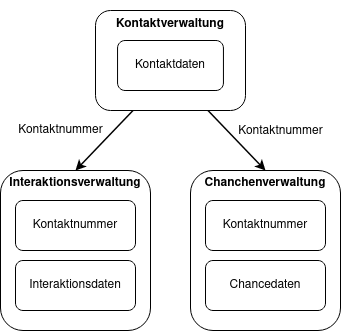
\includegraphics[width=0.65\textwidth]{figures/ContextMap.png}
    \caption{Context Map}
    \label{fig:CRMENTWURF}
\end{figure}

Nachdem die fachliche Einteilung erledigt ist, kann die technische Architektur entworfen werden. Zur flexiblen Skalierbarkeit müssen die Microservices zustandslos sein. Alle persistenten Daten werden also in einer Datenbank abgelegt. Um eine möglichst große Unabhängigkeit zwischen den Microservices zu haben, soll jeder Microservice einer eigenen Datenbank mit einem eigenen Datenbankschema zugeordnet werden. So können die Datenbanken geändert werden, ohne unbeabsichtigte Auswirkungen auf andere Microservices zu haben.

Der Interaktions-Microservice und der Chancen-Microservice benötigen Informationen vom Kontakt-Microservice, damit eine Interaktion beziehungsweise einer Chance ein entsprechender Kontakt zugeordnet werden kann. Zwischen Kontaktverwaltung und Interaktionsverwaltung sowie zwischen Kontaktverwaltung und Chancenverwaltung ist somit eine Kommunikation nötig. Gibt es zu viele solcher Abhängigkeiten oder zyklische Aufrufe, sollte die Einteilung der Microservices überarbeitet werden. Außerdem sollen alle Funktionalitäten auch über eine API angeboten werden. Es bietet sich an, die Kommunikation zwischen den Microservices auch über diese \acp{API} abzuwickeln. 

Um die Microservices klein zu halten soll ein einheitliches und zentrales Frontend entwickelt werden, welches alle Funktionalitäten der Microservices bündelt. Um die Funktionalitäten zu integrieren, greift das Frontend auch auf die \acp{API} der Microservices zu. Somit ergibt sich der folgende Architekturentwurf.

\begin{figure}[H] 
    \centering
    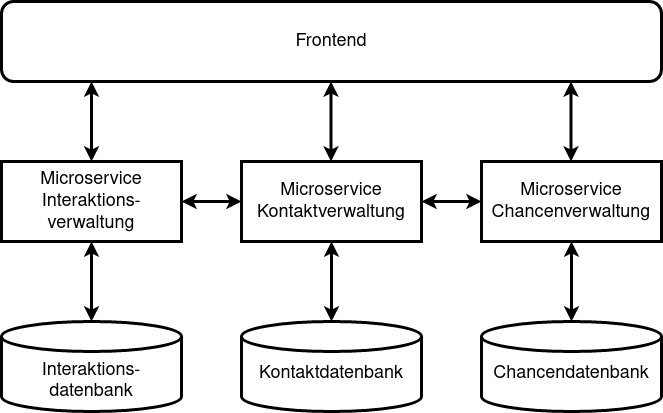
\includegraphics[width=0.71\textwidth]{figures/CRMEntwurf.png}
    \caption{Makro-Architektur des \ac{CRM}-Systems}
    \label{fig:CRMENTWURF}
\end{figure}

Als Nächstes müssen die \acp{API} einheitlich spezifiziert werden. Die \ac{API} wird nach dem \ac{REST}-Architekturstil entworfen. Die Kommunikation erfolgt dabei über \ac{HTTP}. Die \ac{REST}-Ressourcen sollen im \ac{JSON}-Format dargestellt werden. Für jeden Microservice werden die Endpunkte unter der die API aufrufbar ist, die HTTP-Anfragemethode und die zu übergebenden Parameter bestimmt. Wie die einzelnen Ressourcen aufgebaut sind, wird erst in der Mikro-Architektur bestimmt, wenn das Datenmodell der einzelnen Microservices erstellt wurde.

\begin{figure}[H] 
\centering
    \begin{tabular}[H]{|l|l|l|l|}
    		\hline
        \rowcolor{lightgray!50}
        Endpunkt & Methode & Parameter & Beschreibung \\
        \hline
        \hline
        \multicolumn{4}{|c|}{Microservice Kontaktverwaltung} \\
        \hline
        /contacts & GET & - & Gibt alle Kontakte zurück \\
        \hline
        /contacts & POST & neuer Kontakt & Fügt einen neuen Kontakt hinzu \\
        \hline
        /contacts/\{ID\} & GET & - & Gibt einen Kontakt zurück \\
        \hline
        /contacts/\{ID\} & PUT & veränderter Kontakt & Ändert einen Kontakt \\
        \hline
        /contacts/\{ID\} & DELETE & - & Löscht einen Kontakt \\
        \hline
        \hline
        \multicolumn{4}{|c|}{Microservice Interaktionsverwaltung} \\
        \hline
        /interactions & GET & - & Gibt alle Interaktionen zurück \\
        \hline
        /interactions & POST & neue Interaktion & Fügt einen neue Interaktion hinzu \\
        \hline
        /interactions/\{ID\} & GET & - & Gibt eine Interaktion zurück \\
        \hline
        /interactions/\{ID\} & PUT & veränderte Interaktion & Ändert eine Interaktion \\
        \hline
        /interactions/\{ID\} & DELETE & - & Löscht eine Interaktion \\
        \hline
        \hline
        \multicolumn{4}{|c|}{Microservice Chancenverwaltung} \\
        \hline
        /opportunity & GET & - & Gibt alle Chancen zurück \\
        \hline
        /opportunity & POST & neue Chance & Fügt einen neue Chance hinzu \\
        \hline
        /opportunity/\{ID\} & GET & - & Gibt eine Chance zurück \\
        \hline
        /opportunity/\{ID\} & PUT & veränderter Chance & Ändert eine Chance \\
        \hline
        /opportunity/\{ID\} & DELETE & - & Löscht eine Chance \\
        \hline
    \end{tabular}
    \caption{Entwurf der REST-API}
\end{figure}

\subsection{Mikro-Architektur}

Für das Gesamtsystem ist die Architektur eines einzelnen Microservice nicht von Bedeutung. Dadurch besitzt man bei der Gestaltung der Mikro-Architektur viel Freiheit. Bei der Auswahl der Technologien wird auf bewährte und populäre Lösungen gesetzt.

Die drei Microservices werden mit dem selben Technologie-Stack und einer ähnlichen Architektur entworfen, um den Entwicklungsaufwand zu reduzieren. Es wird Java in Verbindung mit dem Spring Boot Framework verwendet. Spring Boot ist beliebteste Framework in Java und durch die einfache Konfiguration gut geeignet für Microservices. Spring Boot ermöglicht eine schnelle Auswahl und Zusammenstellung von gewünschten Abhängigkeiten. Auch REST-APIs werden von Spring Boot natürlich unterstützt. Für die Datenbanken wird MongoDB verwendet. MongoDB ist eine modernes dokumentorientiertes Datenbankmanagementsystem. Daten werden als Dokumente mit einem \ac{JSON}-ähnlichen Aufbau verwaltet. 

Der Entwurf der drei Microservices ist größtenteils analog aufgebaut. Als Erstes werden die Datenmodelle der Microservices modelliert. Zur Modellierung der Datenmodelle werden UML-Klassendiagramme verwendet. UML ist eine grafische Modellierungssprache. Im Laufe der Arbeit werden noch weitere UML-Diagrammarten zum Einsatz kommen. Die Datenmodelle müssen die gewünschten Attribute aus den Anforderungen enthalten.

\begin{figure}[H] 
    \centering
    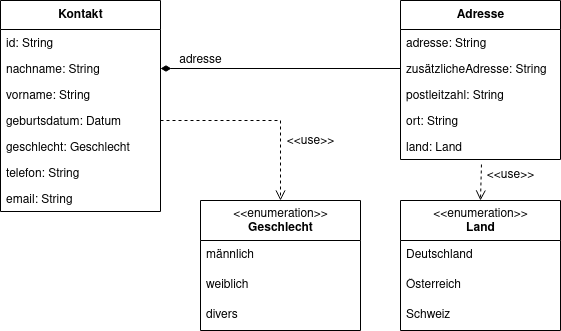
\includegraphics[width=0.71\textwidth]{figures/DatenmodellKontakt.png}
    \caption{Datenmodell Microservice Kontaktverwaltung}
    \label{fig:CRMENTWURF}
\end{figure} 

\begin{figure}[H] 
    \centering
    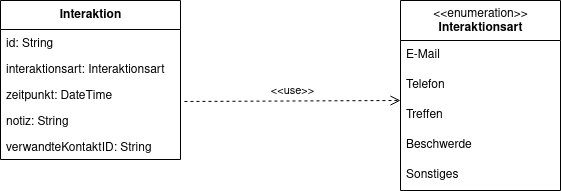
\includegraphics[width=0.71\textwidth]{figures/DatenmodellInteraktion.png}
    \caption{Datenmodell Microservice Interaktionsverwaltung}
    \label{fig:CRMENTWURF}
\end{figure} 

\begin{figure}[H] 
    \centering
    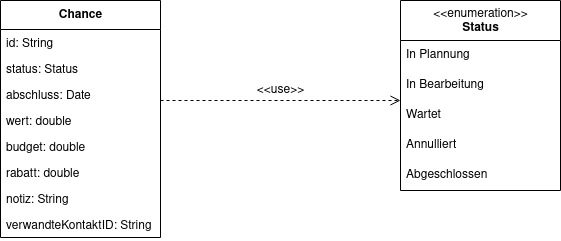
\includegraphics[width=0.71\textwidth]{figures/DatenmodellChance.png}
    \caption{Datenmodell Microservice Chancenverwaltung}
    \label{fig:CRMENTWURF}
\end{figure} 

Dafür wird die JavaScript-Bibliothek React eingesetzt. Es ist derzeit eine der beliebteste Frontendtechnologien. Anwendungen können aus Komponenten zusammengesetzt werden, welche effizient gerendert und aktualisiert werden.

Für das Backend wird Java und das Spring Boot Framework verwendet. Spring Boot ermöglicht eine schnelle und automatische Konfiguration von Abhängigkeiten. Verschiedene Datenbankanbindungen und Unterstützung für REST APIs.


 Die folgenden Domänenmodelle zeigen, welche Daten von den entsprechenden Microservices verwaltet werden müssen.

Das Frontend wird dabei eine clientseitige Webanwendung

\begin{figure}[H] 
    \centering
    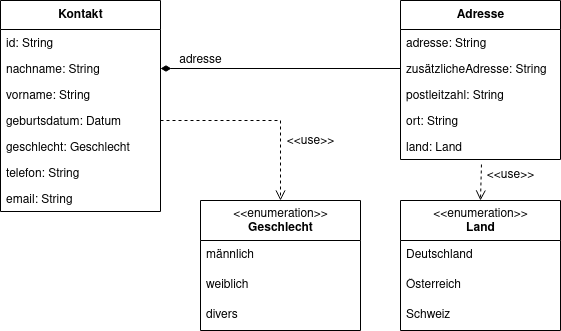
\includegraphics[width=0.71\textwidth]{figures/KontaktUMLDiagram.png}
    \caption{Context Map}
    \label{fig:CRMENTWURF}
\end{figure} 

\begin{figure}[H] 
    \centering
    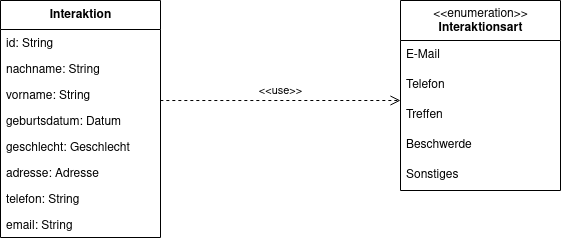
\includegraphics[width=0.71\textwidth]{figures/InteraktionUMLDiagram.png}
    \caption{Context Map}
    \label{fig:CRMENTWURF}
\end{figure} 

\begin{figure}[H] 
    \centering
    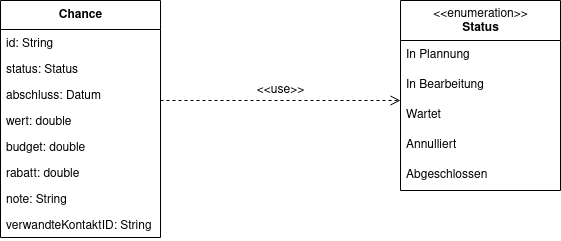
\includegraphics[width=0.71\textwidth]{figures/ChanceUMLDiagram.png}
    \caption{Context Map}
    \label{fig:CRMENTWURF}
\end{figure} 

Für die Architektur der Microservices wird eine hexagonale Architektur (Ports und Adapter) verwendet. Eine Hexagonale Architektur bietet sich 

\begin{figure}[H] 
    \centering
    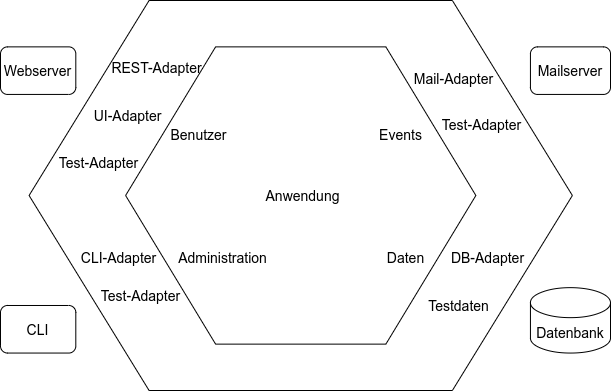
\includegraphics[width=0.71\textwidth]{figures/HexagonalDesignConcept.png}
    \caption{Entwurf des \acp{Hexagonale Architektur}}
    \label{fig:CRMENTWURF}
\end{figure}

\clearpage
\section{Implementierung}


Für das Frontend wird React verwendet. [React Erklärung]
Für alle drei Microservices wird derselbe Technologie-Stack verwendet, um den Entwicklungsaufwand geringer zu halten. Es wird Java mit dem Framework Spring Boot verwendet. Als Datenbank wird MongoDB eingesetzt. [MongoDB Erklärung] Darüber hinaus wird Swagger in die Microservices integriert. Bei Swagger handelt es sich ein Werkzeug zur sprachunabhängigen Spezifikation von APIs. Swagger kann durch eine Abhängigkeit zu Spring Boot hinzu gefügt werden. Es erstellt automatisch eine Webseite mit der Dokumentation unserer API. Um das Monitoring, Service Discovery, Load Balancing wird mit Kubernetes gelöst. Unser System muss diese Aufgaben also nicht selbst bewältigen und diese Bestandteile werden erst in der Bereitstellung konfiguriert.


An dieser Stelle sei auch erwähnt, dass der gesamte Quellcode im folgenden GitHub Repository einsehbar ist: \href{https://github.com/SimonHirner/bachelor-thesis}{github.com/SimonHirner/bachelor-thesis}.

In diesem Kapitel wird das CRM-System dem Entwurf nach implementiert. Als Erstes wird die Implementierung der Microservices erklärt, da alle drei durch den gleichen Technologie-Stack sehr ähnlich sind. Anschließend wird das Frontend, welches alle Microservices integriert, implementiert.

\subsection{Microservices}

Alle drei Microservices benötigen die \ac{URI} ihrer Datenbank, um mit ihr eine Verbindung aufzubauen. Der Interaktions-Microservice und der Verkaufschancen-Microservice brauchen darüber hinaus die Adresse des Kontakt-Microservices, um mit diesem zu Kommunizieren. Diese Verbindungsinformationen, werden den Anwendungen über Umgebungsvariablen übergeben. Später bei der Bereitstellung, kann mit Kubernetes den Containern die passenden Umgebungsvariablen übergeben werden.

\begin{figure}[H] 
    \centering
    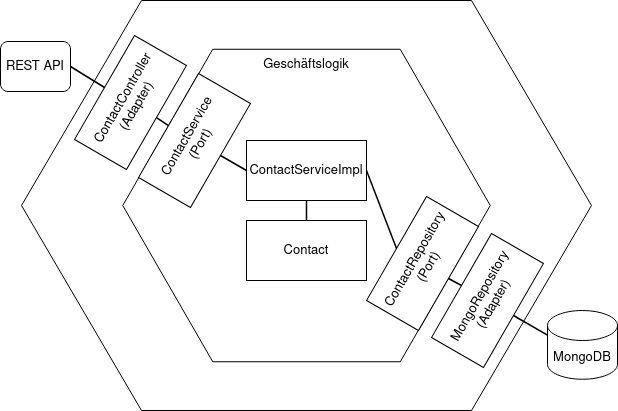
\includegraphics[width=0.71\textwidth]{figures/HexagonalDesign.png}
    \caption{Entwurf des \acp{Hexagonale Architektur}}
    \label{fig:CRMENTWURF}
\end{figure}

\begin{figure}[H] 
    \centering
    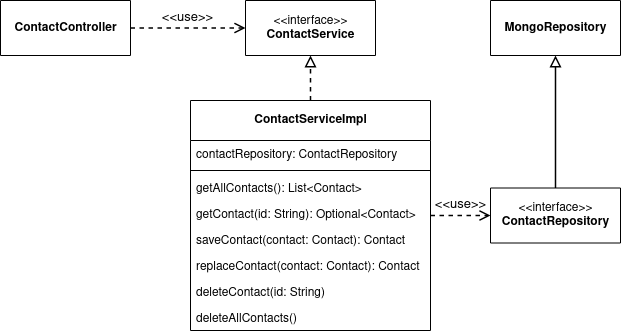
\includegraphics[width=0.71\textwidth]{figures/UMLKlassenDiagram.png}
    \caption{Entwurf des \acp{Hexagonale Architektur}}
    \label{fig:CRMENTWURF}
\end{figure}

\begin{figure}[H] 
    \centering
    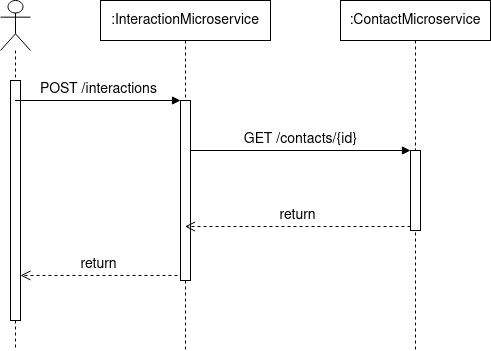
\includegraphics[width=0.71\textwidth]{figures/UMLSequenzdiagramm.png}
    \caption{Entwurf des \acp{Hexagonale Architektur}}
    \label{fig:CRMENTWURF}
\end{figure}

\subsection{Frontend}

Das Frontend. Das Frontend soll später auch mit Kubernetes bereitgestellt werden, es wird aber nicht als Microservices angesehen. Das Frontend benötigt die \ac{URI} aller Services. Auch hier werden die Verbindungsinformationen über eine Umgebungsvariable übergeben.

\clearpage
\section{Bereitstellung mit Kubernetes}

Im letzten Teil des Fallbeispiels wird das fertige CRM-System nun mit Kubernetes bereitgestellt.

\subsection{Containerisierung}

Um die Microservices und das Frontend in Pods in einem Kubernetes Cluster laufen zu lassen, müssen sie erst mit Docker containerisiert werden. Dazu wird als Erstes ein Dockerfile für jeden Microservice erstellt. Anschließend kann aus dem Dockerfile ein Docker Image gebaut werden, mit dem dann ein entsprechender Container gestartet werden kann. \\
\\

Dockerfiles besitzen eine eigene Syntax. Ein großgeschriebener Befehl wird gefolgt von einem oder mehreren Parametern. Es ist aufgebaut wie eine Anleitung, welche Schritt für Schritt abgearbeitet wird. Die Dockerfiles der Microservices haben alle den selben Aufbau, da alle drei Projekte auch die selben Aufbau und die selben Technologien verwenden. Der erste Befehl in den Dockerfiles bestimmt, auf welchem Docker Image unser eigenes Image basieren soll. Hier wird ein Image mit einer Java-Plattform verwendet, welches automatisch aus dem öffentlichen DockerHub heruntergeladen wird. Anschließend wird die JAR-Datei der Anwendung in das Image kopiert. Als letzter Befehl wird festgelegt, dass die JAR-Datei beim Start des Containers ausgeführt werden soll.

\begin{lstlisting}[language=dockerfile, caption=Dockerfile für Kontakt-Microservice]
FROM openjdk:11-jdk-slim
ARG JAR_FILE=target/*.jar
COPY ${JAR_FILE} app.jar
EXPOSE 8080
ENTRYPOINT ["java","-jar","/app.jar"]
\end{lstlisting}

Das Frontend benötigt ein eigenes Dockerfile. Dieses hat einen mehrstufigen Aufbau. Im ersten Stufe, der Build-Stage, wird unsere React-Anwendung gebaut. Um die fertig gebaute Webanwendung an einen Browser auszuliefern wird ein Webserver benötigt. In der zweiten Stufe des Dockerfiles basiert auf einem Image mit dem Webserver Nginx. Die React-Anwendung aus der Build-Stage wird nun in das finale Image kopiert.

\begin{lstlisting}[language=dockerfile, caption=Dockerfile für Frontend]
FROM node:alpine as build
WORKDIR /app
COPY package*.json ./
RUN npm install --silent
COPY . .
RUN npm run build

FROM nginx:alpine
WORKDIR /usr/share/nginx/html
RUN rm -rf ./*
COPY --from=build /app/build .
ENTRYPOINT ["nginx", "-g", "daemon off;"]
\end{lstlisting}

Für die Datenbanken müssen keine eigenen Dockerfiles erstellt werden. Hier reichen unveränderte Images, welche aus dem DockerHub heruntergeladen werden können, aus. Mit dem folgenden Befehl kann aus dem Dockerfile nun ein Docker Image gebaut werden.

\begin{lstlisting}[language=bash, caption=Befehl , captionpos=b]
docker build -t contact-microservice:latest .
\end{lstlisting}


\subsection{Bereitstellung}

Für jede Datenbank wird eine Anwendung 

\begin{figure}[H] 
    \centering
    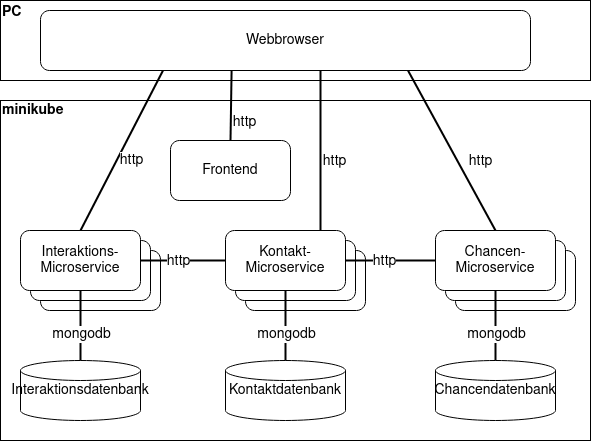
\includegraphics[width=0.71\textwidth]{figures/DeploymentDiagramm.png}
    \caption{Entwurf des \acp{Hexagonale Architektur}}
    \label{fig:CRMENTWURF}
\end{figure}

Jetzt müssen die fertigen Images in unserem Kubernetes Cluster bereitgestellt werden. Dafür werden YAML-Dateien erstellt, in denen die gewünschten Kubernetes Objekte beschrieben werden. Für jeden der drei Microservices und das Frontend muss ein Service und ein Deployment erstellt werden. Das Deployment repräsentiert die Anwendung. Mit Parametern kann festgelegt werden wie viele Pods mit der Anwendung gestartet werden sollen.

\begin{lstlisting}[language=YAML, caption=Befehl]
apiVersion: apps/v1
kind: Deployment
metadata:
  name: contact-service
spec:
  replicas: 1
  template:
    metadata:
      labels:
        app: contact-service
    spec:
      containers:
        - name: contact-service
          image: contact-microservice:latest
          imagePullPolicy: IfNotPresent
          ports:
          - containerPort: 8080
          env:
            - name: MONGODB_HOST
              valueFrom:
                configMapKeyRef:
                  name: contact-db-config  
                  key: host
\end{lstlisting}

\begin{lstlisting}[language=YAML, morekeywords=host, caption=Befehl , captionpos=b]
apiVersion: v1
kind: ConfigMap
metadata:
   name: contact-service-config
data:
 host: contact-service
\end{lstlisting}

Nach der Erstellung der Services wird die Service Discovery und Lasterverteilung von Kubernetes übernommen. 

\begin{lstlisting}[language=YAML, caption=Befehl , captionpos=b]
kind: Service
apiVersion: v1
metadata:
  name: contact-service
spec:
  selector:
    app: contact-service
  ports:
  - protocol: TCP
    port: 8080
    nodePort: 30010
  type: NodePort
\end{lstlisting}

Nun müssen nur noch alle YAML-Dateien über den folgenden kubectl-Befehl angewendet werden. Kubernetes sorg nun dafür, dass die beschriebenen Objekte, erstellt werden.

\begin{lstlisting}[language=bash, caption=Befehl , captionpos=b]
kubectl apply -f contact-microservice.yaml
\end{lstlisting}

\subsection{Skalierung}

Um die Vorteile von unseren Microservices auszunutzen, sollen die Microservices nun horizontal skaliert werden. Auch dafür wird eine YAML-Datei erstellt, in der ein HorizontalPodAutoscaler-Objekt für jeden Microservice beschrieben wird. In der Datei wird angegeben, welches Deployment skaliert werden soll. Als Metrik, wann hochskaliert werden soll, kann die CPU-Auslastung des Pods verwendet werden. Darüber hinaus wird angegeben wie viele Pods von dem entsprechenden Microservice minimal und maximal ausgeführt werden sollen.

\begin{lstlisting}[language=YAML, caption=Befehl , captionpos=b]
apiVersion: autoscaling/v1
kind: HorizontalPodAutoscaler
metadata:
    name: contact-service
spec:
    scaleTargetRef:
        apiVersion: apps/v1
        kind: Deployment
        name: contact-service
    minReplicas: 2
    maxReplicas: 4
    targetCPUUtilizationPercentage: 80
\end{lstlisting}
